\documentclass[11pt]{article}

% Change "review" to "final" to generate the final (sometimes called camera-ready) version.
% Change to "preprint" to generate a non-anonymous version with page numbers.
\usepackage[review]{acl}

% Standard package includes
\usepackage{times}
\usepackage{latexsym}

% For proper rendering and hyphenation of words containing Latin characters (including in bib files)
\usepackage[T1]{fontenc}
% For Vietnamese characters
% \usepackage[T5]{fontenc}
% See https://www.latex-project.org/help/documentation/encguide.pdf for other character sets

% This assumes your files are encoded as UTF8
\usepackage[utf8]{inputenc}

% This is not strictly necessary, and may be commented out,
% but it will improve the layout of the manuscript,
% and will typically save some space.
\usepackage{microtype}

% This is also not strictly necessary, and may be commented out.
% However, it will improve the aesthetics of text in
% the typewriter font.
\usepackage{inconsolata}

%Including images in your LaTeX document requires adding
%additional package(s)
\usepackage{graphicx}
\usepackage{booktabs}
\usepackage{amsmath}

% If the title and author information does not fit in the area allocated, uncomment the following
%
%\setlength\titlebox{<dim>}
%
% and set <dim> to something 5cm or larger.

\title{Position Confounds Attention: Re-evaluating Attention-Based\\ Object Hallucination Detectors in Vision--Language Models}

% Author information can be set in various styles:
% For several authors from the same institution:
% \author{Author 1 \and ... \and Author n \\
%         Address line \\ ... \\ Address line}
% if the names do not fit well on one line use
%         Author 1 \\ {\bf Author 2} \\ ... \\ {\bf Author n} \\
% For authors from different institutions:
% \author{Author 1 \\ Address line \\  ... \\ Address line
%         \And  ... \And
%         Author n \\ Address line \\ ... \\ Address line}
% To start a separate ``row'' of authors use \AND, as in
% \author{Author 1 \\ Address line \\  ... \\ Address line
%         \AND
%         Author 2 \\ Address line \\ ... \\ Address line \And
%         Author 3 \\ Address line \\ ... \\ Address line}

\author{First Author \\
  Affiliation / Address line 1 \\
  Affiliation / Address line 2 \\
  Affiliation / Address line 3 \\
  \texttt{email@domain} \\\And
  Second Author \\
  Affiliation / Address line 1 \\
  Affiliation / Address line 2 \\
  Affiliation / Address line 3 \\
  \texttt{email@domain} \\}

%\author{
%  \textbf{First Author\textsuperscript{1}},
%  \textbf{Second Author\textsuperscript{1,2}},
%  \textbf{Third T. Author\textsuperscript{1}},
%  \textbf{Fourth Author\textsuperscript{1}},
%\\
%  \textbf{Fifth Author\textsuperscript{1,2}},
%  \textbf{Sixth Author\textsuperscript{1}},
%  \textbf{Seventh Author\textsuperscript{1}},
%  \textbf{Eighth Author \textsuperscript{1,2,3,4}},
%\\
%  \textbf{Ninth Author\textsuperscript{1}},
%  \textbf{Tenth Author\textsuperscript{1}},
%  \textbf{Eleventh E. Author\textsuperscript{1,2,3,4,5}},
%  \textbf{Twelfth Author\textsuperscript{1}},
%\\
%  \textbf{Thirteenth Author\textsuperscript{3}},
%  \textbf{Fourteenth F. Author\textsuperscript{2,4}},
%  \textbf{Fifteenth Author\textsuperscript{1}},
%  \textbf{Sixteenth Author\textsuperscript{1}},
%\\
%  \textbf{Seventeenth S. Author\textsuperscript{4,5}},
%  \textbf{Eighteenth Author\textsuperscript{3,4}},
%  \textbf{Nineteenth N. Author\textsuperscript{2,5}},
%  \textbf{Twentieth Author\textsuperscript{1}}
%\\
%\\
%  \textsuperscript{1}Affiliation 1,
%  \textsuperscript{2}Affiliation 2,
%  \textsuperscript{3}Affiliation 3,
%  \textsuperscript{4}Affiliation 4,
%  \textsuperscript{5}Affiliation 5
%\\
%  \small{
%    \textbf{Correspondence:} \href{mailto:email@domain}{email@domain}
%  }
%}

\begin{document}
\maketitle
\begin{abstract}
Training-free detectors of object hallucination in large vision--language models (LVLMs) increasingly rely on attention signals, and report strong area-under-ROC (AUROC) on caption-level benchmarks. We show that much of this performance is an artifact of \emph{generation-position confounding}: in autoregressive captioning, both visual attention mass and hallucination rate vary systematically with how far into the caption a token appears, so a detector can score well by tracking position rather than grounding. We introduce a position-controlled evaluation protocol---within-bin, matched-pair, and residual AUROC---that holds generation position fixed. On LLaVA-1.5-7B over MSCOCO ($16{,}426$ object mentions), generation position alone reaches $0.830$ AUROC. Under position control, attention-mass detectors (PAS, SVAR) retain only $22$--$28\%$ of their above-chance signal, dropping from $\sim$$0.83$ overall to $\sim$$0.58$ within-bin, whereas representation- and uncertainty-based detectors (Internal Confidence, output entropy) remain position-robust ($0.69$ and $0.64$ within-bin). To test whether \emph{any} carefully engineered attention-shape feature survives, we build SinkDetect, which scores the purified shape of the visual attention distribution (sink removal, top-mass masking, cross-layer consistency); even so, its within-bin AUROC collapses to chance. We argue that overall AUROC is misleading for this task and that position-controlled evaluation should be standard.
\end{abstract}

\section{Introduction}

Large vision--language models (LVLMs) such as LLaVA-1.5 \cite{PLACEHOLDER_liu2023llava} produce fluent image captions, but routinely \emph{hallucinate}: they mention objects that are not present. Detecting these hallucinated mentions---ideally at the token level, without retraining---has become an active research target, and a growing line of work derives detection scores from the model's internal \emph{attention}: how much, and where, the object token attends over the image \cite{jiang2024devils,hoangxuan2026pas}. Such detectors report strong caption-level AUROC and are attractive because they are training-free and computable during inference.

We argue that these reported numbers are systematically inflated by a confound that the standard evaluation ignores: \textbf{the generation position of the object token}. Captions are produced autoregressively. As generation proceeds, two things happen at once. First, the model attends progressively less to the image and more to the previously generated text---visual attention mass decays with position. Second, hallucinations become far more frequent late in the caption: on our data the per-token hallucination rate rises from $2.2\%$ in the first ten generated tokens to over $60\%$ past position 100. Position is therefore a common cause of both the attention signal and the label. A detector that merely reads off ``how much this token attends to the image'' will appear to detect hallucination while in fact tracking position.

This confound is not hypothetical. On LLaVA-1.5-7B over MSCOCO, a trivial detector that uses \emph{only} the generation position index achieves $0.830$ AUROC---higher than every attention-based baseline we evaluate. Any method whose overall AUROC sits near or below this value has not been shown to contribute grounding-specific signal at all.

\paragraph{Contributions.} We make the case that attention-based hallucination detection must be evaluated with position held fixed, and we show what survives when it is.

\begin{itemize}
\item We identify generation-position confounding in token-level LVLM hallucination detection and quantify it: position alone reaches $0.830$ AUROC (\S\ref{sec:confound}).
\item We introduce a \textbf{position-controlled evaluation protocol}---within-bin, matched-pair, and residual AUROC---that isolates position-independent signal, and re-evaluate nine baselines under it (\S\ref{sec:protocol},~\S\ref{sec:results}).
\item We show a clean split: attention-mass detectors (PAS, SVAR) retain only $22$--$28\%$ of their above-chance signal, while representation/uncertainty detectors (Internal Confidence, entropy, NLL) remain position-robust (\S\ref{sec:results}).
\item As a stress test, we build \textbf{SinkDetect}, a detector designed specifically to read the \emph{shape} (not the mass) of purified visual attention. Its within-bin AUROC still collapses to chance, providing evidence that the limitation is structural to attention-magnitude signals rather than an artifact of crude feature engineering (\S\ref{sec:sinkdetect}).
\end{itemize}

\section{Related Work}

\paragraph{Object hallucination detection in LVLMs.} We organize prior detectors by the \emph{signal source} they read, because this axis turns out to predict robustness to the confound we study. (i)~\textbf{Uncertainty} detectors use the output distribution at the object step: the negative log-likelihood (NLL) or the entropy of the next-token distribution. They are cheap and model-agnostic but can miss confident hallucinations. (ii)~\textbf{Representation} detectors read internal hidden states: Internal Confidence (IC) projects image representations into the vocabulary and measures the support assigned to the object \cite{jiang2024interpreting}, while GLSim compares global and local image--text embedding similarity \cite{park2025glsim}. (iii)~\textbf{Attention} detectors read the object token's attention over the image: SVAR sums a visual-attention ratio across layers \cite{jiang2024devils}, PAS measures attention diverted to previously generated ``prelim'' tokens \cite{hoangxuan2026pas}, and Beyond-Global-Scores combines attention dispersion (ADS) with cross-modal grounding consistency (CGC) at the patch level \cite{beyond2026global}. The field has trended from uncertainty to representation to ever finer attention signals, and reports steadily higher overall AUROC over CHAIR-derived labels \cite{PLACEHOLDER_rohrbach2018chair}. Our contribution is orthogonal: rather than proposing a detector to top this leaderboard, we re-evaluate the families under position control and ask which signal source carries position-independent information.

\paragraph{Position and length effects.} Two facts are individually known: LVLMs hallucinate more as a caption lengthens, and visual attention attenuates as autoregressive decoding proceeds. Their \emph{joint} consequence for evaluation has been overlooked. Because both the label and attention-derived features move with position, aggregate AUROC cannot tell whether a detector tracks grounding or merely tracks how far into the caption a token sits. We make this confound explicit, quantify it, and fold it into the evaluation protocol. Methodologically, holding a nuisance variable fixed (binning, matching, residualization) is standard practice in observational analysis; our contribution is to import it into hallucination-detection benchmarking, where it has been absent.

\section{Generation-Position Confounding}
\label{sec:confound}

Let an object mention be a generated token at position $p$ (counted from the first generated token). Each mention has a binary hallucination label $y$ from CHAIR. We observe two position-dependent trends on LLaVA-1.5-7B / MSCOCO (\S\ref{sec:setup}):

\begin{enumerate}
\item \textbf{Label shift.} The hallucination rate $\Pr(y{=}1\mid p)$ rises monotonically with $p$, from $0.022$ at $p\in[0,10)$ to $>0.60$ at $p>100$.
\item \textbf{Feature shift.} Attention-mass features (e.g., total visual attention) decay with $p$ as decoding shifts weight toward generated text.
\end{enumerate}

When a feature and the label share position as a common cause, a detector can achieve high AUROC by exploiting position rather than grounding. Concretely, position $p$ acts as a confounder $p \rightarrow s$ and $p \rightarrow y$ for any score $s$ whose distribution shifts with $p$; the induced association between $s$ and $y$ is then partly or wholly spurious. We confirm the confound is strong: a logistic detector using only $p$ attains $0.830$ overall AUROC (Table~\ref{tab:main}, ``Position-only''). This sets a floor: \emph{overall AUROC near or below $0.830$ is not evidence of grounding-specific signal.}

\paragraph{Mechanism (TODO figure).} We will add a figure plotting mean total visual-attention mass against generation position, split by hallucinated vs.\ grounded mentions, to visualize the feature shift that drives the confound. The decay curve is the intended ``anchor'' figure of the paper; the plotting script is implemented but the final vector figure is not yet included here.

\section{Position-Controlled Evaluation}
\label{sec:protocol}

We propose three complementary metrics that hold position fixed. Let $\{(s_i, y_i, p_i)\}_{i=1}^N$ be the detector scores, labels, and generation positions over $N$ object mentions, with $s$ oriented so that higher means more likely hallucinated. Let $\mathrm{AUROC}(S)$ denote the standard area under the ROC curve computed over an index set $S$. The three metrics differ only in how they neutralize $p$.

\paragraph{Within-bin AUROC.} Partition the positions into bins $B_1,\dots,B_K$ of width $10$. Within each bin compute $a_k = \mathrm{AUROC}(B_k)$, discarding bins with fewer than two label classes or $<10$ samples, and report the size-weighted mean $\sum_k |B_k| a_k / \sum_k |B_k|$. This measures discrimination among tokens \emph{at the same position}.

\paragraph{Matched-pair AUROC.} For each hallucinated mention, pair it with the position-nearest grounded mention. Report the fraction of pairs in which the hallucinated token receives the higher score (ties count $0.5$). This is a paired analogue robust to bin-edge effects.

\paragraph{Residual AUROC.} Regress $s$ on $p$ (and likewise the label) and evaluate AUROC on the residuals, removing the linear position component.

A detector whose signal is purely positional scores $\approx$$0.5$ on all three, regardless of its overall AUROC. A detector with genuine grounding signal retains a value well above $0.5$.

\section{Experimental Setup}
\label{sec:setup}

\paragraph{Model and data.} We use LLaVA-1.5-7B \cite{PLACEHOLDER_liu2023llava} on the MSCOCO val2014 split \cite{PLACEHOLDER_lin2014coco}, generating detailed captions with the standard prompt. Object mentions are labeled hallucinated/grounded by CHAIR against COCO ground-truth objects \cite{PLACEHOLDER_rohrbach2018chair}. This yields $16{,}426$ object mentions ($4{,}009$ hallucinated, $12{,}417$ grounded). All baselines are evaluated on the same generations and labels.

\paragraph{Baselines.} We reproduce nine detectors spanning the three families: NLL and entropy (uncertainty); Internal Confidence (IC) and GLSim with its global/local variants (representation); SVAR and PAS (attention). We additionally report Beyond-ADS, Beyond-CGC, and their combination (fine-grained patch grounding). PAS and GLSim follow their authors' released formulations; Beyond-Global-Scores is reimplemented from its description as no official code was available at the time of writing.

\paragraph{TODO (planned for camera-ready).} The current draft uses a single model and dataset. To support the generality claim we plan to add: (i) $\geq$2 further LVLMs (e.g., InstructBLIP, Qwen-VL); (ii) Objects365 as a second dataset; (iii) a causal check via position-matched null distributions and intervention. These are not yet run and \emph{no numbers for them appear in this draft}.

\section{Results}
\label{sec:results}

\begin{table*}[t]
\centering
\small
\begin{tabular}{llcccc}
\toprule
Method & Family & Overall & Within-bin & Matched-pair & Residual \\
\midrule
\multicolumn{2}{l}{\emph{Position-only}} & 0.830 & --- & --- & --- \\
\midrule
NLL            & Uncertainty    & 0.711 & 0.636 & 0.652 & 0.630 \\
Entropy        & Uncertainty    & 0.721 & 0.637 & 0.654 & \textbf{0.634} \\
IC             & Representation & 0.776 & \textbf{0.686} & \textbf{0.703} & 0.633 \\
GLSim          & Representation & 0.723 & 0.541 & 0.556 & 0.565 \\
GLSim (global) & Representation & 0.620 & 0.506 & 0.505 & 0.511 \\
GLSim (local)  & Representation & 0.772 & 0.564 & 0.593 & 0.601 \\
SVAR           & Attention      & 0.834 & 0.575 & 0.576 & 0.557 \\
PAS            & Attention      & \textbf{0.835} & 0.593 & 0.583 & 0.569 \\
Beyond-ADS     & Patch grounding& 0.503 & 0.511 & 0.515 & 0.501 \\
Beyond-CGC     & Patch grounding& 0.692 & 0.521 & 0.520 & 0.518 \\
Beyond-ADS+CGC & Patch grounding& 0.693 & 0.523 & 0.524 & 0.521 \\
\bottomrule
\end{tabular}
\caption{Overall vs.\ position-controlled AUROC on LLaVA-1.5-7B / MSCOCO ($16{,}426$ mentions). Generation position alone reaches $0.830$. Attention-mass detectors (PAS, SVAR) have the highest overall AUROC but collapse under position control; representation/uncertainty detectors (IC, Entropy, NLL) remain robust. Best per column in \textbf{bold}.}
\label{tab:main}
\end{table*}

\begin{figure*}[t]
\centering
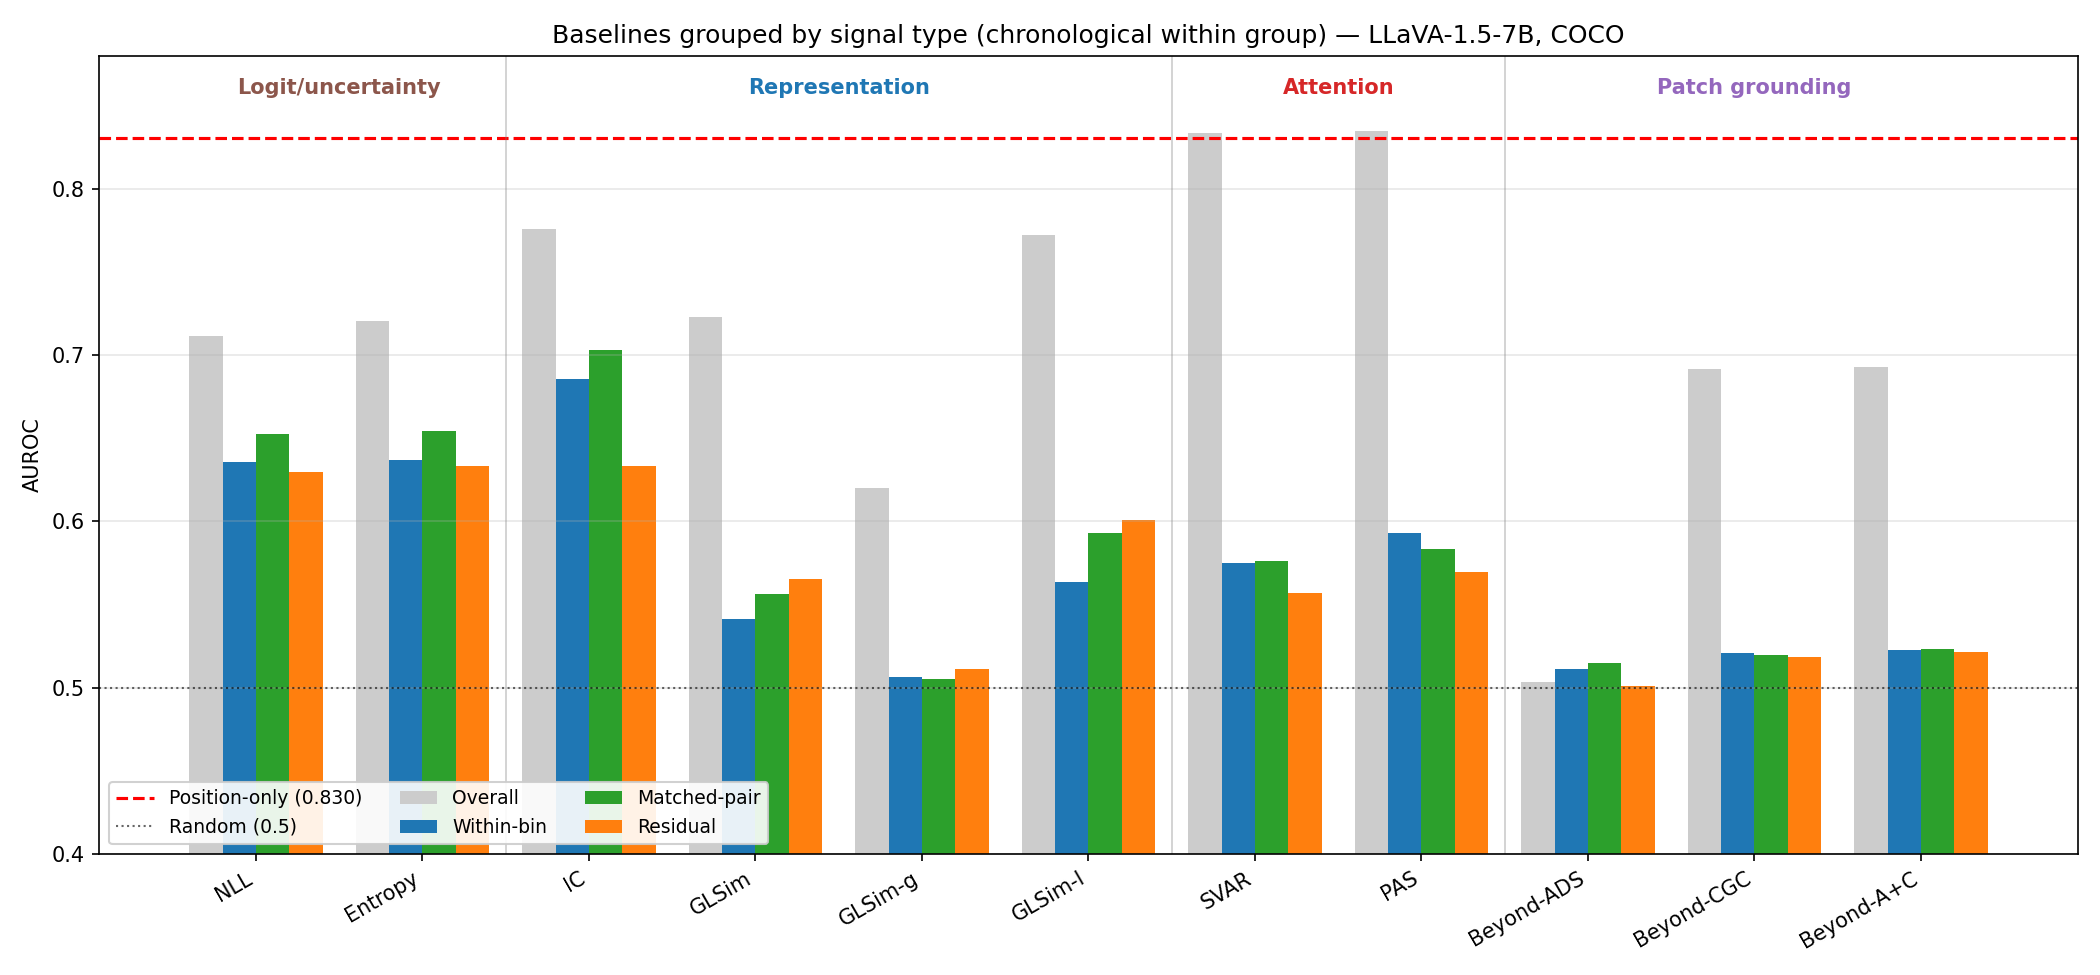
\includegraphics[width=0.95\textwidth]{figures/fig_summary.png}
\caption{Overall vs.\ position-controlled AUROC, grouped by signal family (chronological within group). The dashed line marks position-only AUROC ($0.830$); the dotted line marks chance ($0.5$). For PAS and SVAR the gray (overall) bars touch the position-only line, but the position-controlled bars drop to $\sim$$0.58$, indicating their discriminative power is largely positional.}
\label{fig:summary}
\end{figure*}

\begin{figure*}[t]
\centering
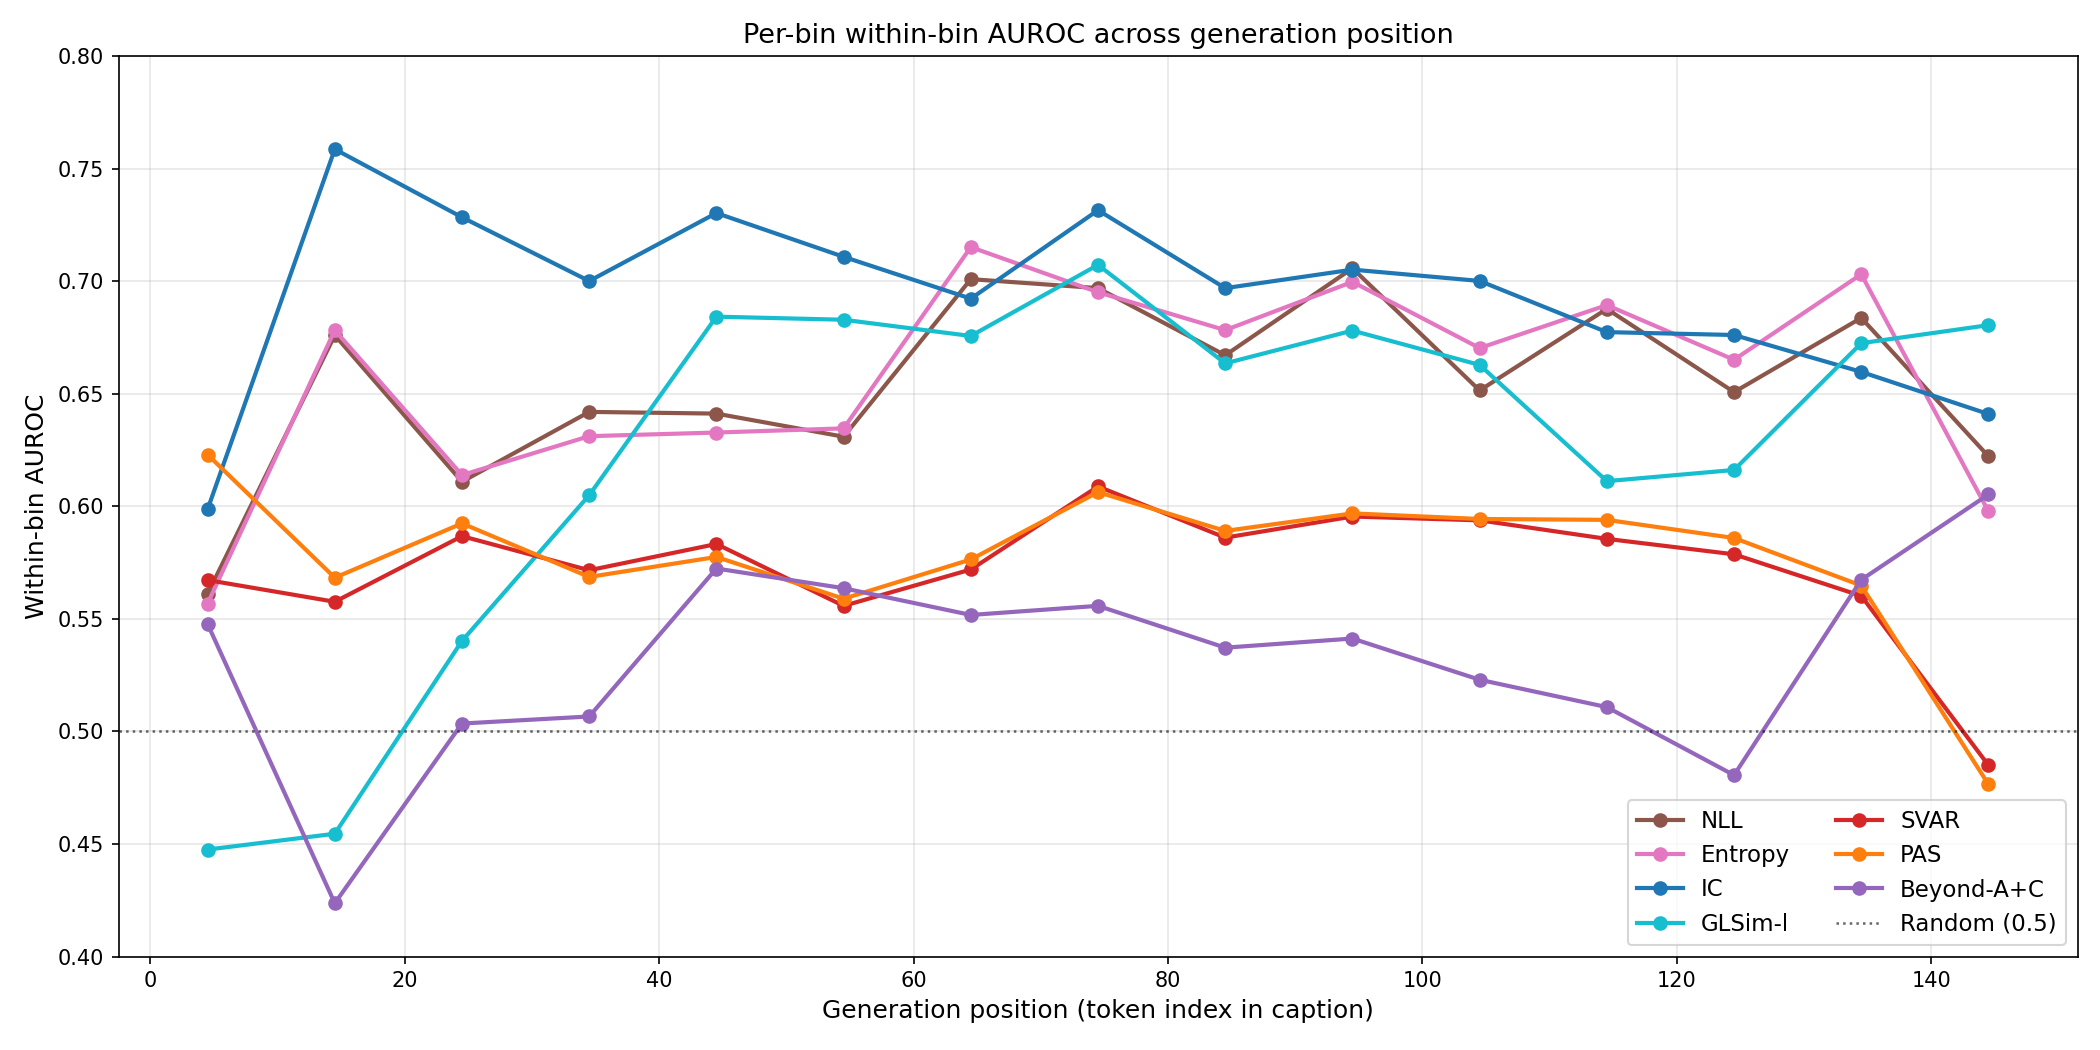
\includegraphics[width=0.95\textwidth]{figures/fig_per_bin.png}
\caption{Within-bin AUROC across generation position (bin width $10$). IC stays highest and most stable ($0.66$--$0.76$); NLL/Entropy follow; PAS/SVAR sit near $0.55$--$0.60$; Beyond-ADS+CGC is near chance throughout.}
\label{fig:perbin}
\end{figure*}

\paragraph{A clean split between families.} Table~\ref{tab:main} and Figure~\ref{fig:summary} show that overall AUROC and position-controlled AUROC tell opposite stories for the attention family. PAS and SVAR have the two \emph{highest} overall AUROCs ($0.835$, $0.834$)---at or above the position-only floor---yet their within-bin AUROC is only $0.593$ and $0.575$. Expressed as retained above-chance signal, $(\text{within-bin}-0.5)/(\text{overall}-0.5)$, PAS keeps $28\%$ and SVAR $22\%$. By contrast, IC keeps $67\%$ ($0.686$ within-bin), entropy $62\%$, and NLL $64\%$. The fine-grained patch-grounding detectors (Beyond-*) are near chance on all position-controlled metrics. There is essentially no middle ground: methods retain either $\sim$$60$--$67\%$ or $\sim$$12$--$28\%$.

\paragraph{The split tracks signal source, not recency.} Ordering methods by proposal date (Figure~\ref{fig:summary}) shows the earliest representation method, IC, remains the strongest position-controlled detector, ahead of every later attention/grounding method. Improvements in overall AUROC over time largely reflect better fitting of the position prior, not new position-independent signal.

\paragraph{Per-position view.} Figure~\ref{fig:perbin} confirms the gap is consistent across positions: IC dominates in nearly every bin, whereas PAS/SVAR remain flat near $0.55$--$0.60$ throughout. The advantage of representation/uncertainty signals is not concentrated in a few easy bins.

\section{Stress Test: SinkDetect}
\label{sec:sinkdetect}

A natural objection is that attention \emph{shape}, as opposed to attention \emph{mass}, might carry position-independent grounding signal that prior attention detectors simply read too crudely. To test this directly we build SinkDetect, a detector designed to read shape.

\paragraph{Method.} Let $\tilde a_q$ be the object query's attention row restricted to the visual-token span, with detected sink columns removed and the remainder $L_1$-normalized to a distribution. SinkDetect scores $\tilde a_q$ along three axes. \emph{(i) Counterfactual visual grounding (CVG):} the negative divergence $-\mathrm{KL}(\tilde a_q \,\|\, \pi)$ and $-\mathrm{JSD}(\tilde a_q, \pi)$ from null distributions $\pi$ taken as the average instruction-token attention, a uniform distribution, and a local non-object null; closeness to a language-prior null is treated as evidence of hallucination. \emph{(ii) Concentration:} the entropy $H(\tilde a_q)$ and top-$k$ mass, testing whether attention is diffuse. \emph{(iii) Cross-layer consistency (CLC):} the generalized Jensen--Shannon divergence among the per-layer distributions, testing whether the attended region is stable across depth. Sinks are visual tokens with anomalously large pre-RoPE key norm that absorb attention mass without carrying semantics; removing them, together with an optional top-mass mask, forms a $2\times2$ purification ablation, each variant optionally recomputed on a no-RoPE branch. The full score set spans these axes $\times$ purification variants $\times$ per-layer/global aggregation. Crucially, because every distribution is $L_1$-normalized before scoring, total attention mass---the position-confounded quantity---is divided out by construction; SinkDetect therefore isolates \emph{shape}.

\paragraph{Result.} Despite this design, SinkDetect's best within-bin AUROC is $\approx$$0.50$, and its residual AUROC is $0.49$--$0.51$. Its highest \emph{overall} AUROC ($0.81$) again comes from a concentration score that correlates with position. Normalizing away mass does not help, because the confound also lives in the \emph{shape} of the normalized distribution: early tokens attend broadly (high entropy), late tokens attend narrowly, independent of grounding. We read this as evidence that the limitation is structural to attention-magnitude--derived signals on this model, not a failure of feature engineering: even purpose-built shape features, with sinks and dominant patches removed, recover no position-independent signal.

\section{Discussion}

Our findings do not show that attention is irrelevant to grounding; they show that the \emph{aggregate visual-attention statistics} used by current detectors are dominated by generation position. Two readings remain open and we cannot yet distinguish them: either per-token grounding signal is absent from these attention summaries, or it is present but washed out by averaging over heads, layers, and the normalized distribution. That IC recovers $0.69$ within-bin from representations---which the attention mechanism feeds---suggests object-level information does exist internally; locating it inside attention (e.g., specific heads/layers) is left to future work.

\section*{Limitations}

This draft reports a single model (LLaVA-1.5-7B) and a single dataset (MSCOCO). The central claim---that attention-mass detectors are position-confounded while representation/uncertainty detectors are robust---is demonstrated only in this setting; multi-model and multi-dataset replication (Section~\ref{sec:setup}, TODO) is required before the claim can be stated as general, and is planned for the camera-ready. We establish a strong \emph{correlational} confound but not yet a causal one; the planned position-matched-null and intervention experiments are intended to close this gap. Position is one confounder (likely the dominant one) but not necessarily the only one. Finally, Beyond-Global-Scores is a reimplementation and may underperform an official release. We do not propose a new state-of-the-art detector; the contribution is a corrected evaluation and the finding it surfaces.

\section*{Acknowledgments}

Anonymized for review.

% Custom bibliography entries only
\bibliography{custom}

\appendix

\section{Per-bin AUROC table}
\label{sec:appendix}
A full per-bin breakdown (AUROC for every method in every position bin) accompanies the released code and reproduces Figure~\ref{fig:perbin}.

\end{document}
